\documentclass{rapportECL}
\usepackage{lipsum}
\usepackage{overpic}
\usepackage{xcolor}
\usepackage{graphicx}
\usepackage{tcolorbox}
\usepackage[utf8]{inputenc}
\usepackage[T1]{fontenc}
\usepackage[french]{babel}
\usepackage{amsmath}
\usepackage{amsfonts}
\usepackage{amssymb}
\usepackage{geometry}
\usepackage{listings}
\usepackage{xcolor}
\usepackage{hyperref}
\usepackage{siunitx}      % Pour les unités avec \SI
\usepackage{float}        % Pour le placement [H] des figures

\begin{document}

%----------- Informations du rapport ---------

\titre{Étude et optimisation topologique d’un piston} %Titre du fichier .pdf
% \UE{ DIMENSIONNEMENT DES STRUCTURES} %Nom de la UE
\enseignant{Frédérick \textsc{Bonnavand} \\ Ahmad \textsc{Daniel}} %Nom de l'enseignant


\eleves{BIAOU \textsc{Adebayo Landry}\\ Kevin \textsc{TONGUE}\\ 
VICENT \textsc{Lucie} \\ Gaston \textsc{KAMDEM TCHOMTHOUA} }
\UE{ENISE-5GM}


% \eleves{Kevin \textsc{TONGUE} }
\UEU{ENISE-4GM}

%----------- Initialisation -------------------
        
\fairemarges %Afficher les marges
\fairepagedegarde %Créer la page de garde
\tabledematieres %Créer la table de matières
%============================================================


\section{Introduction}

L'\textbf{optimisation topologique} est une méthode de conception avancée qui vise à améliorer les performances mécaniques d'une pièce tout en réduisant sa masse. Cette approche est particulièrement adaptée à la fabrication additive, laquelle offre une grande liberté géométrique pour réaliser des formes complexes issues de l'optimisation.
\\\\
Dans le cadre du cours\textit{ "Conception pour la Fabrication Additive"}, l'objectif de ce projet est d'optimiser un piston de moteur à combustion interne afin d'en diminuer la masse tout en garantissant sa résistance mécanique sous les chargements imposés. Pour mener cette étude, nous avons utilisé le logiciel \textbf{3D Experience} et ses modules \textbf{Structural}, qui fournissent des outils de simulation et d'analyse structurelle performants.
\\\\
À partir de la géométrie complète du piston, nous avons identifié les zones de matière peu sollicitées et proposé une nouvelle conception allégée, respectant à la fois les contraintes mécaniques et les spécificités de la fabrication additive. Cette démarche permet d'explorer des configurations innovantes, en tenant compte des efforts appliqués et des possibilités de réalisation, afin d'obtenir une structure à la fois légère et performante.

\section{Analyse du besoin et cahier des charges}

\subsection{Objectif de l’étude}

L’objectif de ce projet est de concevoir un piston de moteur à combustion interne aussi léger que possible, tout en garantissant sa résistance mécanique sous les charges appliquées. 
\\\\
L’optimisation vise à réduire la masse en supprimant la matière non essentielle, sans compromettre la tenue structurelle de la pièce. La géométrie finale devra également être compatible avec les contraintes de la fabrication additive.

\begin{figure}[H]
    \centering
    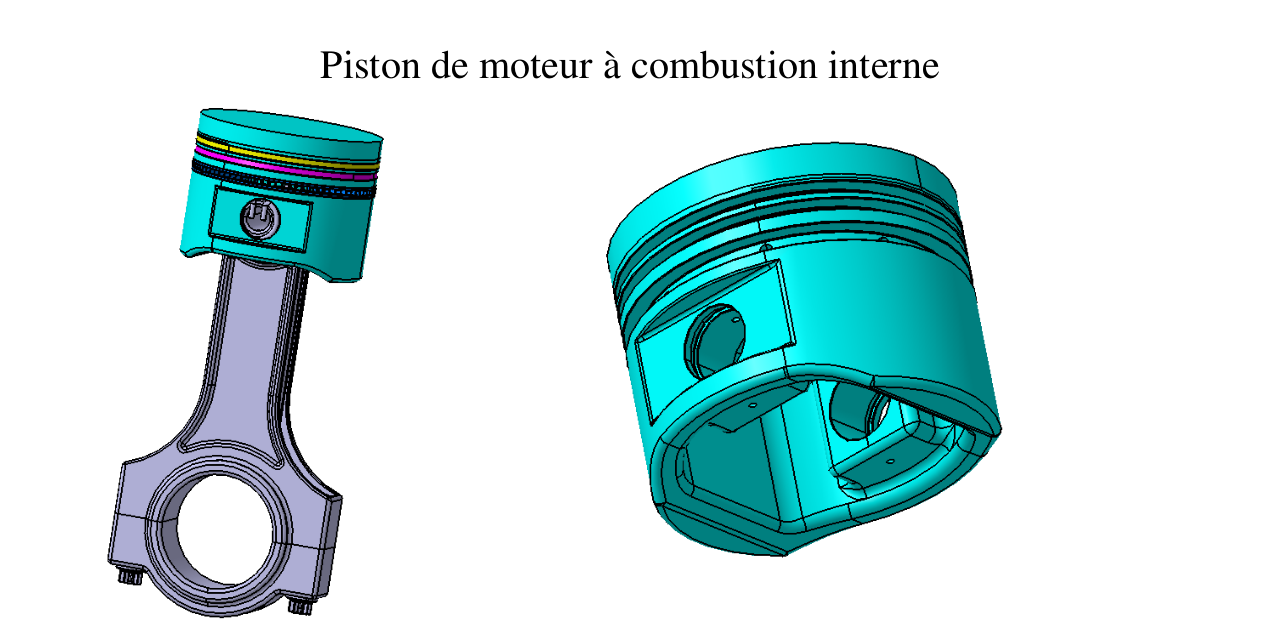
\includegraphics[width=0.9\linewidth]{optimisation_1.png}
    \caption{Géométrie initiale du piston étudié}
    \label{fig:piston_initial}
\end{figure}
\label{sec:cahier}

\textbf{\textit{Afin de définir correctement le problème d’optimisation, il est nécessaire de préciser les fonctions mécaniques du piston ainsi que les chargements, les conditions aux limites et le matériau retenus pour la modélisation.}}

\subsection{Fonctions de la pièce}

Le piston est un organe mécanique fondamental du moteur à combustion interne. Il assure plusieurs fonctions essentielles au bon fonctionnement du système :

\begin{itemize}
    \item \textbf{Transmission des efforts :} il transmet à la bielle, via l’axe de piston, la force résultant de la pression des gaz de combustion appliquée sur sa tête ;
    
    \item \textbf{Guidage cinématique :} il assure le mouvement alternatif rectiligne à l’intérieur du cylindre tout en maintenant un alignement correct avec celui-ci ;
    
    \item \textbf{Étanchéité de la chambre de combustion :} en association avec les segments, il limite les fuites de gaz vers le carter et contribue au maintien de la compression.
\end{itemize}


\subsection{Chargements et conditions aux limites}

La tête du piston est soumise à une pression uniforme maximale de \SI{100}{bars} 
(\SI{10}{MPa}), représentant l’action des gaz de combustion. 
Cette pression est modélisée comme un chargement statique équivalent pour l’étude d’optimisation.
\\\\
Les conditions aux limites sont définies par un appui au niveau des bossages d’axe, 
simulant la liaison avec la bielle, et un guidage radial au niveau de la jupe, 
représentant le contact avec le cylindre.

\subsection{Matériau}
Le matériau est un alliage d'aluminium dont les caractéristiques à \SI{250}{\celsius} sont :
\begin{itemize}
    \item Limite élastique : \(\sigma_e = \SI{120}{MPa}\)
    \item Module d'Young : \(E = \SI{72000}{MPa}\)
    \item Coefficient de Poisson : \(\nu = 0,34\)
\end{itemize}

\section{Présentation de la géométrie initiale}
\label{sec:initiale}

La géométrie de depart est un modèle CAO classique de piston, illustré Figure~\ref{fig:initiale}. Il comprend une tête épaisse, des bossages pour l'axe, une jupe cylindrique et des nervures de rigidification. Cette forme servira de domaine de conception pour l'optimisation topologique.
 
\begin{figure}[H]
    \centering
    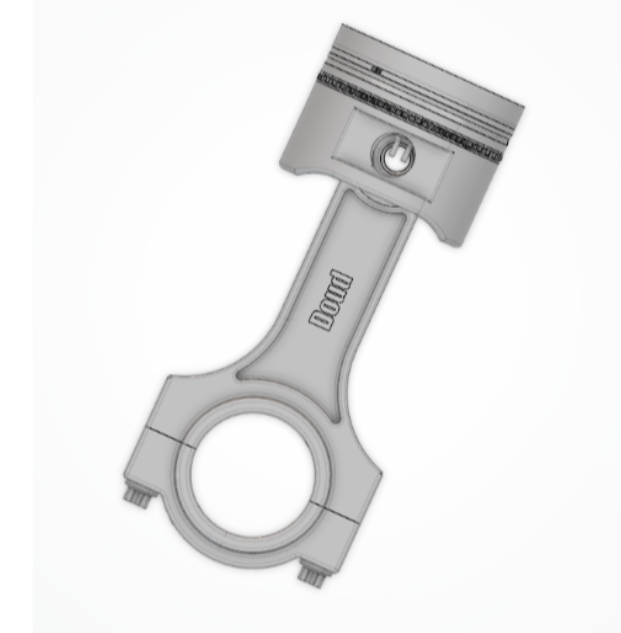
\includegraphics[width=0.6\textwidth]{ioptimisation1.png}
    \caption{Géométrie complet du piston}
    \label{fig:initiale}
\end{figure}

\section{Méthodologie d'optimisation topologique}
\label{sec:methodo}

La démarche d'optimisation topologique mise en œuvre dans ce projet suit un processus itératif en plusieurs étapes, schématisé ci-après. À partir d'une analyse mécanique du concept initial (forme générale), une optimisation topologique est réalisée pour déterminer la distribution optimale de matière. Un seuillage permet ensuite de ne conserver que les éléments les plus sollicités, avant une optimisation paramétrique et une optimisation de forme pour affiner les détails locaux. Enfin, une étape de validation par simulation mécanique vérifie la conformité de la géométrie finale vis-à-vis des critères de performance et de fabricabilité.


\begin{figure}[H]
    \centering
    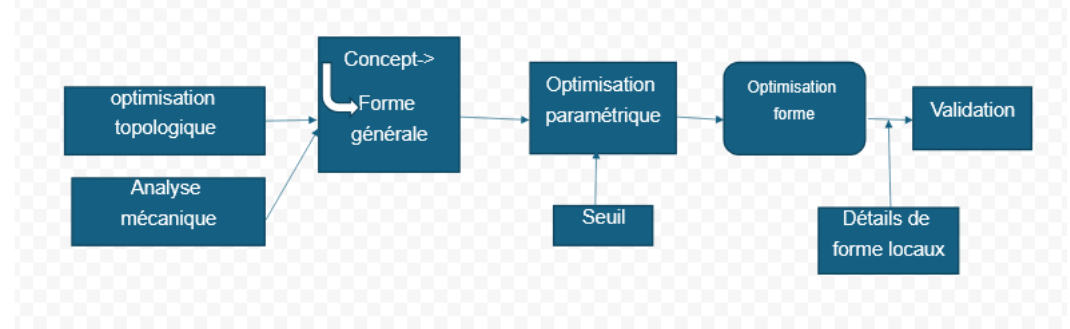
\includegraphics[width=1\linewidth]{ioptimisation2.png}
    \caption{Démarche générale d'optimisation topologique adoptée pour la conception du piston.}
    \label{fig:placeholder}
\end{figure}

\subsection{Analyse mécanique}

Une analyse mécanique préliminaire a été réalisée sur SolidWork afin d'identifier les zones fortement sollicitées du piston et de définir les conditions aux limites ainsi que les chargements appliqués (pression de \SI{100}{bars} sur la tête).

\begin{figure}[H]
    \centering
    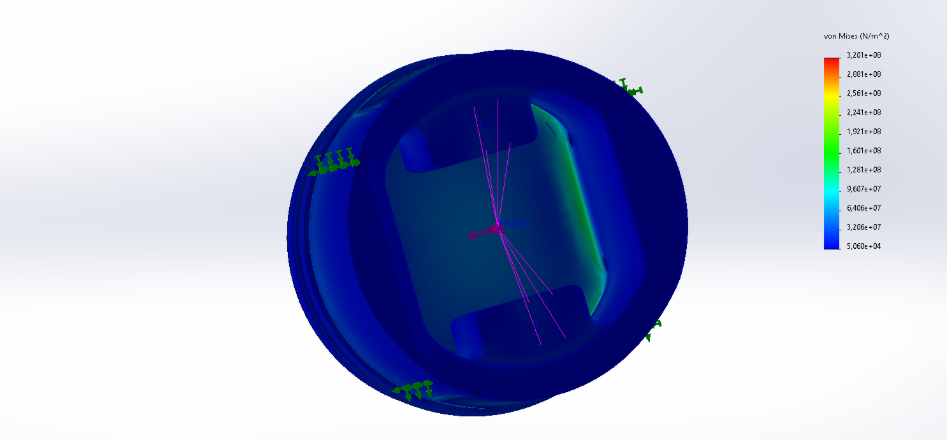
\includegraphics[width=1\linewidth]{ioptimisation3.png}
    \caption{}
    \label{fig:placeholder}
\end{figure}


\begin{figure}[H]
    \centering
    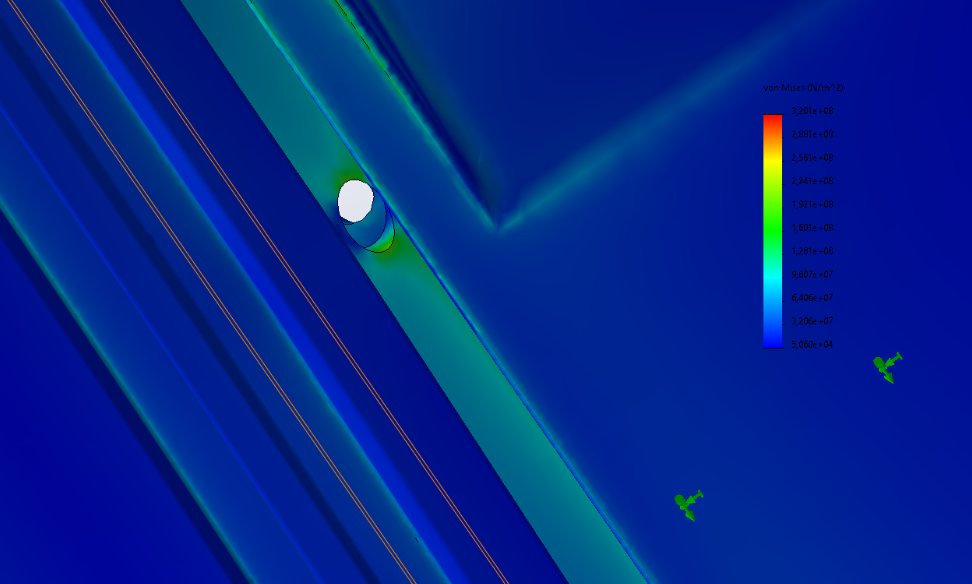
\includegraphics[width=1\linewidth]{ioptimisation4.png}
    \caption{}
    \label{fig:placeholder}
\end{figure}

\subsubsection{Interprétation des résultats de simulation mécanique}

La simulation montre que la contrainte maximale atteint \SI{320}{MPa} sur la chemise du piston, ce qui dépasse largement la limite élastique de \SI{120}{MPa}. Cela entraîne une plastification locale (déformations irréversibles), donc la géométrie actuelle n'est pas adaptée et nécessite une optimisation.


\subsection{Optimisation et simulation du piston}

Après avoir simulé le piston sur SolidWorks, une simulation a également été réalisée sur 3DEXPERIENCE pour analyser les contraintes et identifier les zones critiques à optimiser.

\begin{figure}[H]
    \centering
    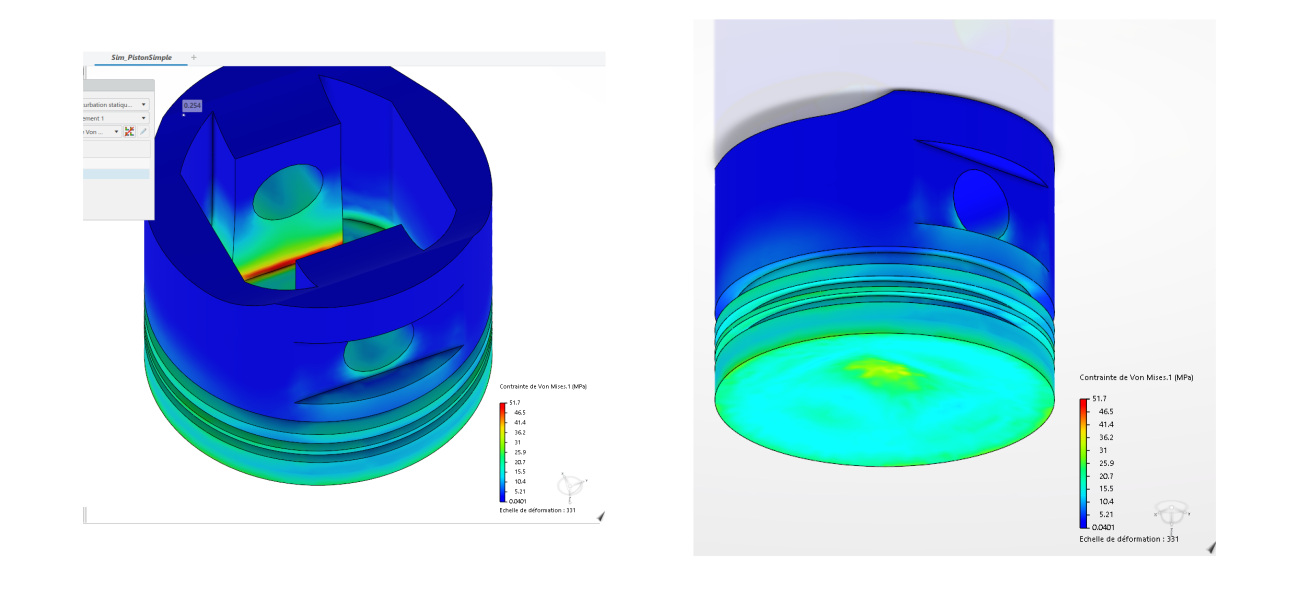
\includegraphics[width=1\linewidth]{ioptimisation5.png}
    \caption{Simulation du piston}
    \label{fig:placeholder}
\end{figure}

\textit{Dans la suite, nous avons réalisé une optimisation topologique de notre piston initial. Nous obtenons avec cette optimisation une contrainte maximale de \SI{105}{MPa}, ce qui est inférieur à la contrainte limite de \SI{120}{MPa}.}


\begin{figure}[H]
    \centering
    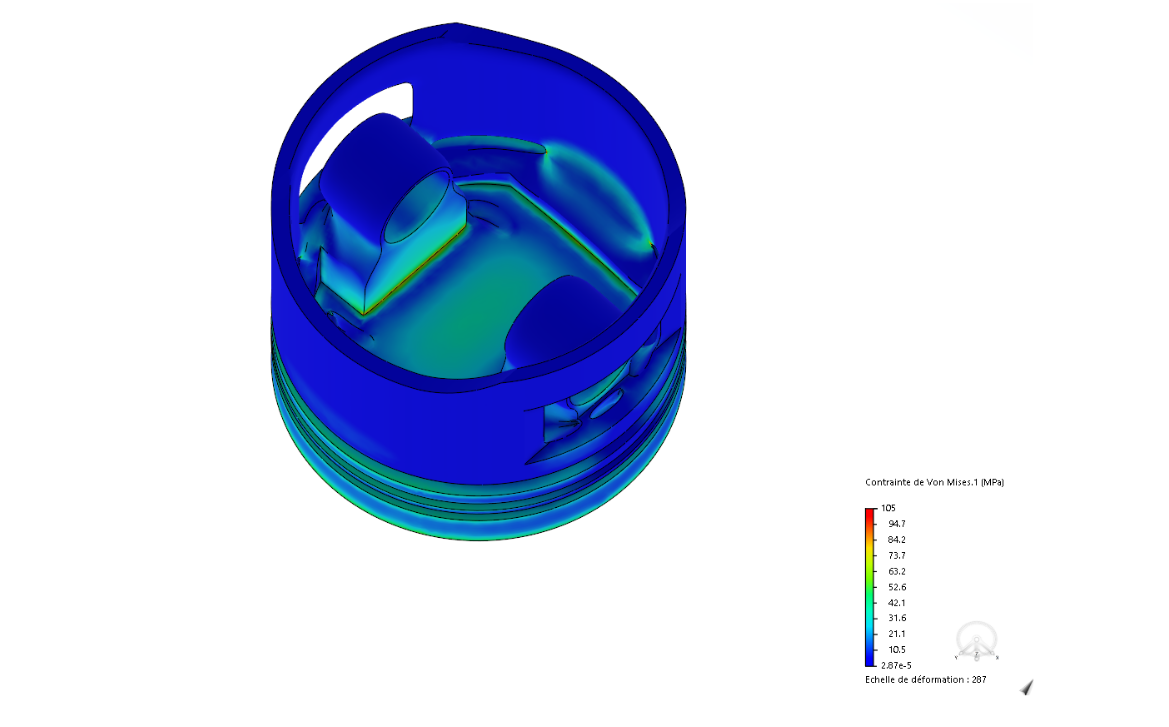
\includegraphics[width=0.7\linewidth]{ioptimisation6.png}
    \caption{Simulation du piston obtenu par optimisation topologique}
    \label{fig:placeholder}
\end{figure}

Pour réduire la contrainte dans la zone entourée en rouge, nous proposons d'ajouter une nervure locale. Cette nervure permettra de mieux répartir les efforts mécaniques et de diminuer la concentration de contraintes. Une simulation ultérieure vérifiera que cette modification respecte toujours la limite d'élasticité de \SI{120}{MPa}, tout en conservant le gain de masse obtenu par l'optimisation topologique. 
\\\\

Dans la suite de notre étude, nous avons conçu une nouvelle forme de piston en nous appuyant sur les principes de l'optimisation topologique. Cette approche nous a permis d'identifier et d'éliminer les zones de matière non essentielles tout en maintenant une résistance mécanique optimale.

\begin{figure}[H]
    \centering
    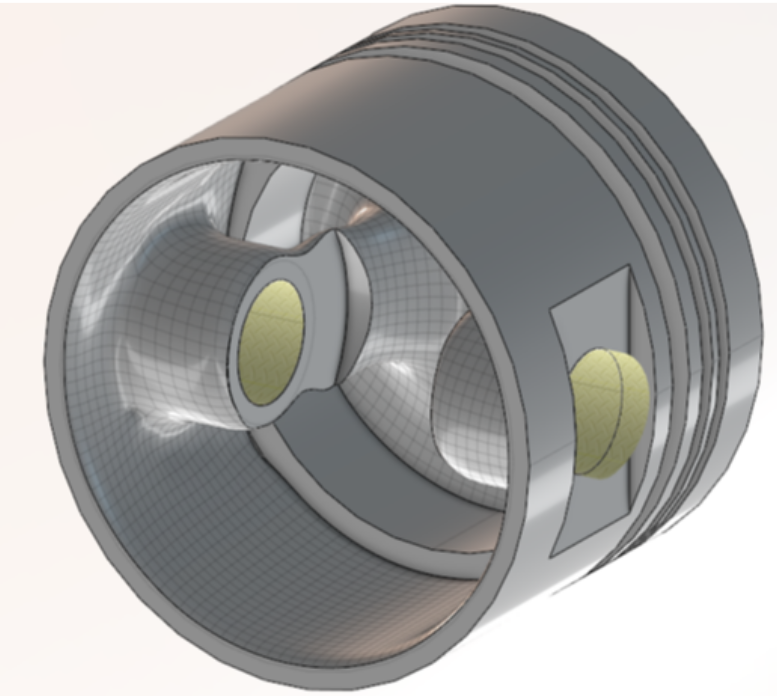
\includegraphics[width=0.5\linewidth]{ioptimisation7.png}
    \caption{}
    \label{fig:placeholder}
\end{figure}

Afin d'évaluer les performances de cette nouvelle conception, nous avons procédé à une simulation numérique à l'aide du logiciel \textit{3D Experience}, notamment avec ses modules d'analyse structurelle. L'objectif de cette simulation est de vérifier si les contraintes mécaniques appliquées sur le piston restent inférieures à la limite élastique du matériau utilisé.


\begin{figure}[H]
    \centering
    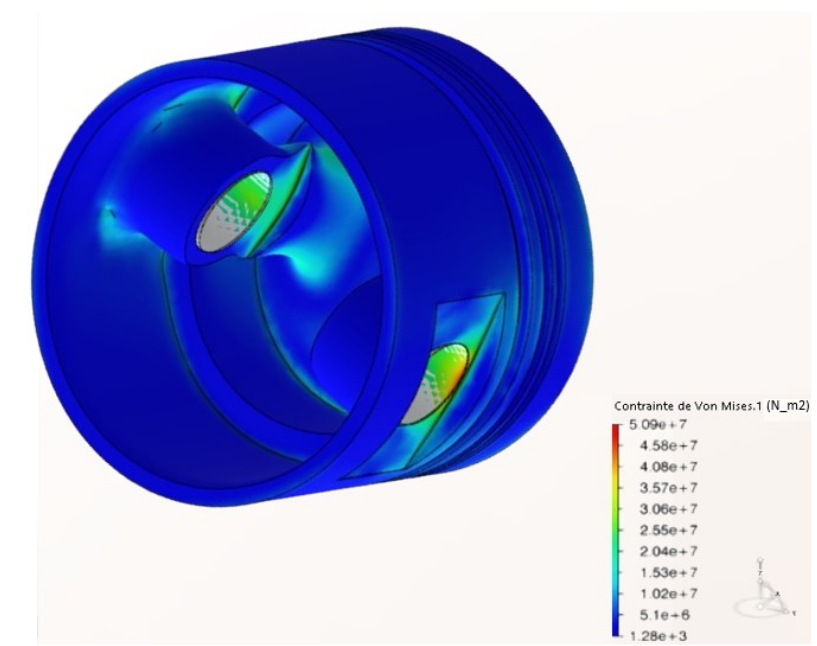
\includegraphics[width=0.5\linewidth]{ioptimisation9.png}
    \caption{}
    \label{fig:placeholder}
\end{figure}


La simulation numérique de la nouvelle conception du piston révèle une contrainte maximale de \SI{5.09e7}{N/m^2} (\SI{50.9}{MPa}), valeur largement inférieure à la limite élastique de \SI{120}{MPa}. Ce résultat confirme que la structure reste dans le domaine élastique, validant ainsi l'efficacité de l'optimisation topologique qui a permis de réduire la masse tout en préservant les performances mécaniques. La marge de sécurité importante offre également des perspectives d'allègement supplémentaire.

Pour poursuivre l'optimisation, une approche manuelle peut être envisagée, par exemple en perçant des trous dans les zones peu sollicitées afin de réduire encore la masse. Une nouvelle simulation devra toutefois vérifier que la contrainte maximale reste inférieure à la limite élastique, garantissant ainsi la résistance et la durabilité du piston en conditions réelles.


\section{Forme simplifiée}
\label{sec:resultats}

\subsection{Simulation}

Cependant, dans la suite du projet, nous avons choisi de modifier directement la géométrie du piston afin de simplifier les calculs et de réduire le temps de simulation. En effet, la géométrie initiale comprend des détails complexes (gorges de segments, trous d'huile) et des pièces hors du cadre de notre étude, ce qui alourdit inutilement les calculs. Une géométrie simplifiée permet d'obtenir des résultats plus rapidement tout en conservant une précision suffisante pour valider la conception optimisée.



\begin{figure}[H]
    \centering
    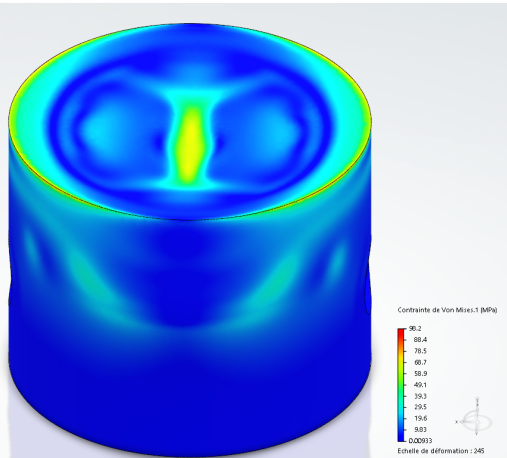
\includegraphics[width=0.6\linewidth]{ioptimisation8.png}
    \caption{Contrainte Von Mises}
    \label{fig:placeholder}
\end{figure}


L'analyse actuelle révèle que la contrainte maximale subie par le piston est de \SI{98.2}{MPa}, ce qui reste inférieur à la limite d'élasticité du matériau. Dans la suite du projet, une optimisation topologique sera mise en œuvre afin d'affiner davantage la conception en identifiant les zones où la matière peut être supprimée sans compromettre la résistance mécanique.

Une fois cette optimisation réalisée, une nouvelle simulation sera effectuée pour évaluer la performance de la pièce modifiée.

\begin{figure}[H]
    \centering
    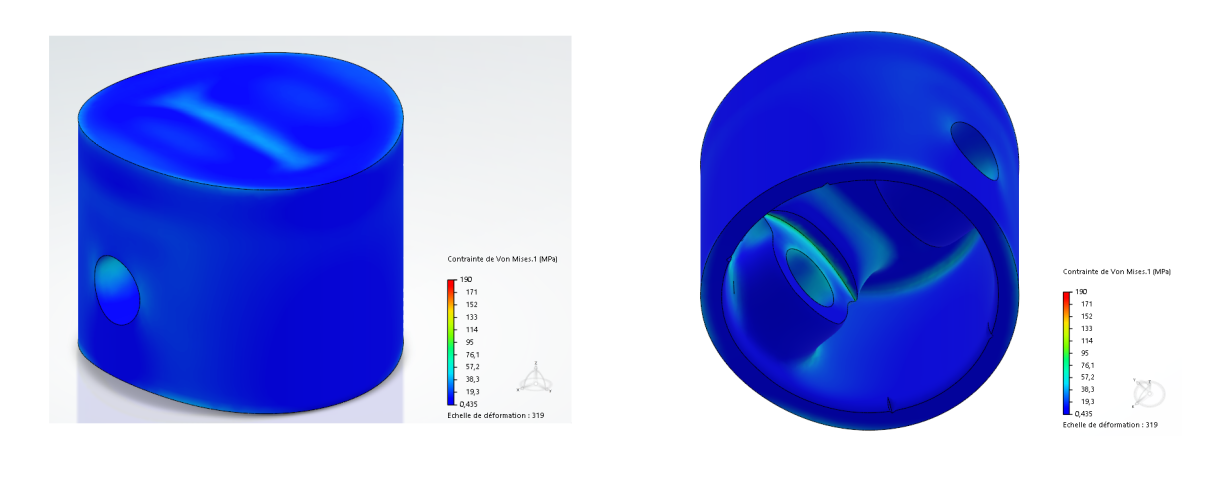
\includegraphics[width=1\linewidth]{ioptimisation10.png}
    \caption{}
    \label{fig:placeholder}
\end{figure}

Après simulation de la nouvelle forme optimisée, les résultats indiquent une contrainte maximale d'environ \SI{114}{MPa}, valeur inférieure à la limite élastique de l'aluminium (\SI{120}{MPa}). Ce résultat valide l'efficacité de l'optimisation topologique : la pièce a été allégée tout en conservant une résistance suffisante. Toutefois, une analyse plus approfondie pourrait être menée pour détecter d'éventuelles concentrations de contraintes. Une optimisation manuelle pourrait également permettre de réduire encore la masse sans dépasser la limite élastique.

\subsection{Optimisation topologique}

Une première optimisation topologique a été réalisée avec un maillage de \SI{3}{mm}, en adoptant une stratégie de minimisation de la masse.


\begin{figure}[h!]
    \centering
    \begin{minipage}{0.45\linewidth}
        \centering
        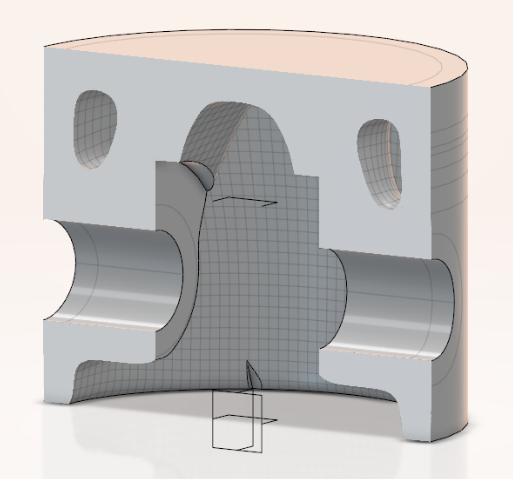
\includegraphics[width=\linewidth]{ioptimisation11.png}
        \caption{Forme optimisation 1}
        \label{fig:optimisation1}
    \end{minipage}\hfill
    \begin{minipage}{0.45\linewidth}
        \centering
        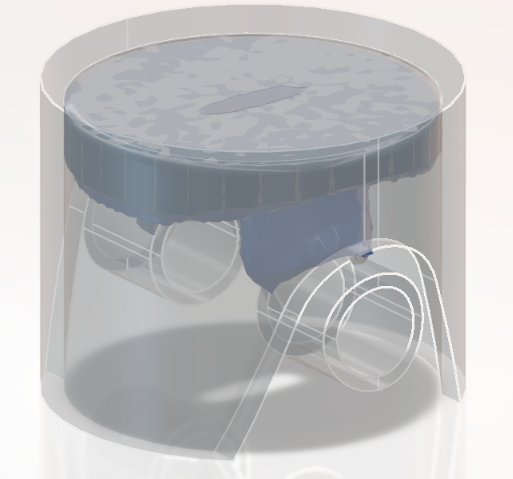
\includegraphics[width=\linewidth]{ioptimisation12.png}
        \caption{Forme optimisation 2}
        \label{fig:optimisation2}
    \end{minipage}
\end{figure}



Une deuxième tentative d'optimisation topologique a été réalisée avec un maillage de \SI{1.5}{mm}, en adoptant une stratégie de minimisation de la masse sous contrainte. Cette approche semblait prometteuse et aurait permis un gain de masse d'environ \SI{60}{\%}. Cependant, un bug logiciel sur \textit{3D Experience} nous a empêchés de modifier certains paramètres et de finaliser cette optimisation.

\begin{figure}[h!]
    \centering
    \begin{minipage}{0.45\linewidth}
        \centering
        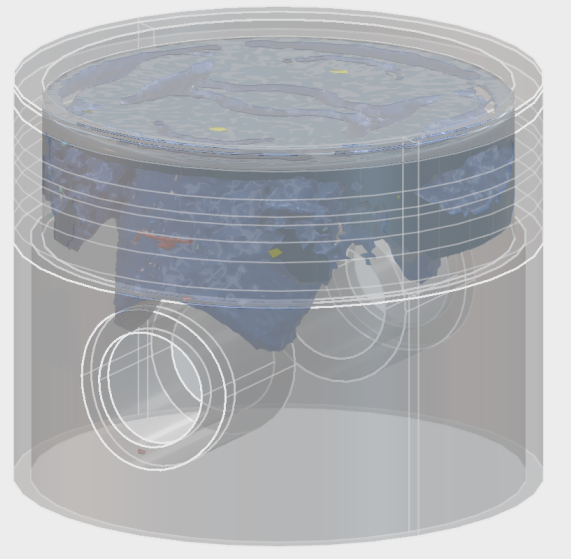
\includegraphics[width=\linewidth]{ioptimisation13.png}
        \caption{Forme optimisation 1}
        \label{fig:optimisation1}
    \end{minipage}\hfill
    \begin{minipage}{0.45\linewidth}
        \centering
        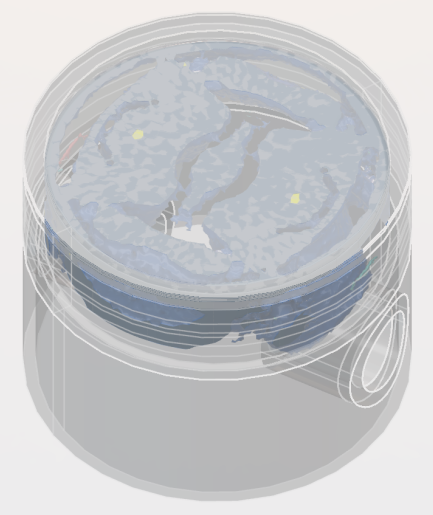
\includegraphics[width=\linewidth]{ioptimisation14.png}
        \caption{Forme optimisation 2}
        \label{fig:optimisation2}
    \end{minipage}
\end{figure}
\newpage

\subsection{Difficultés rencontrées lors des simulations}

Cependant, lors de nos simulations, nous avons rencontré plusieurs difficultés liées au maillage et aux itérations, principalement en raison de la complexité géométrique du modèle. La présence de détails fins, de transitions abruptes et de zones à forte courbure a rendu la génération d'un maillage adapté plus délicate. De plus, des problèmes de convergence ont été observés au cours des itérations : certaines simulations ne parvenaient pas à atteindre un état d'équilibre stable, entraînant des erreurs numériques ou des temps de calcul excessifs. Ces difficultés sont principalement dues aux fortes variations de contraintes dans certaines zones et aux discontinuités géométriques, ce qui complique l'analyse par éléments finis.
\\\\
Pour remédier à ces difficultés, plusieurs stratégies peuvent être envisagées :
\begin{itemize}
    \item [$\bigstar$] Affiner localement le maillage dans les zones critiques tout en conservant un maillage plus grossier ailleurs, afin de limiter la charge de calcul.
    \item [$\bigstar$] Simplifier la géométrie en supprimant certains détails non essentiels qui perturbent la génération du maillage.
    \item [$\bigstar$] Utiliser des algorithmes d'adaptation de maillage qui permettent d'ajuster dynamiquement la taille des éléments en fonction des contraintes observées.
    \item [$\bigstar$] Ajuster les paramètres d'itération du solveur afin d'améliorer la stabilité et la convergence des calculs.
\end{itemize}

\section{Conclusion}
\label{sec:conclusion}

L'optimisation topologique menée sur le piston a permis de réduire significativement sa masse tout en maintenant les contraintes en dessous de la limite élastique. Les simulations ont validé l'efficacité de la conception, avec une meilleure répartition des efforts et un allègement notable. Malgré quelques difficultés liées au maillage et à la convergence, cette étude démontre l'intérêt de l'optimisation topologique pour concevoir des pièces à la fois légères et résistantes, adaptées à la fabrication additive.

\end{document}